\label{chap.3}
\section {Chapter Introduction}
This chapter will introduce the proposed methodology on how to approach the challenge of early plant disease detection and identification by implementing AI and DL approaches. It references the study based on literature and points out how the proposed program meets the need for contemporary research in eliminating the deficits and barriers present. Finally, the chapter highlights the novelty and uniqueness of the proposed framework to be not only resource-friendly but also user-friendly to the nonscientific individual.
\section{Proposed Work}
% Provide an overview of the proposed work, connecting it to the research gaps identified in the Literature Study chapter.
% Briefly restate the problem.
% Highlight how your proposed work addresses the gaps or challenges.
% Emphasize the novelty or uniqueness of your approach.

Modern agricultural methods face severe challenges that arise from plant diseases, leading to a decrease in crop production and monetary loss. Early diagnosis of plant diseases is thus very critical to overcome such impacts. However, available methods are resource-intensive, require expert intervention, and are not scalable. The purpose of our proposed study is to develop an artificial intelligence-based system that helps detect plant diseases early, but with low resource intensity and infrastructure requirements. The focus should be on developing a solution that is cost-effective, user-friendly, and easily accessible to farmers and agriculturalists, especially those who are in remote or resource-limited areas.

\

Through an extensive review of existing literature and current methodologies in plant disease detection systems, several critical gaps and limitations have been identified that significantly impact the practical implementation and accessibility of these solutions. A primary concern is the heavy reliance on sophisticated and expensive equipment, including high-resolution imaging systems, specialized sensors, and advanced computational hardware. This dependence on costly infrastructure creates a substantial barrier for small-scale farmers and agricultural communities with limited resources, effectively excluding a significant portion of the target user base from accessing these technological advancements. Furthermore, the existing solutions demonstrate a notable limitation in dataset diversity, with many systems being developed and trained on narrow, crop-specific datasets. This specialization, while potentially beneficial for specific applications, severely restricts the systems' generalizability and adaptability across different agricultural contexts and varied crop types. The challenge of real-time analysis presents another significant hurdle, as numerous existing systems operate primarily through offline processing mechanisms, introducing considerable delays between disease detection and implementation of remedial measures. This delay can be critical in agricultural scenarios where rapid response is essential for disease containment and crop preservation. The complexity in deployment represents another substantial barrier, with many current solutions requiring extensive technical expertise and sophisticated computational resources for successful implementation. This technical complexity makes these systems particularly impractical for deployment in rural and remote agricultural areas, where technical support and infrastructure may be limited. Additionally, scalability emerges as a crucial concern, as few existing approaches have successfully developed frameworks that can be readily adapted and scaled across different crop varieties and disease types while maintaining accuracy and efficiency. The integration challenges with contemporary mobile and web-based platforms further compound these limitations, as many systems lack user-friendly interfaces and accessible deployment options that would make them practical tools for farmers and agricultural workers. These technological and accessibility barriers collectively highlight the pressing need for more inclusive, scalable, and practically implementable solutions in plant disease detection systems.

\

The research initiative seeks to fill critical gaps in the detection of agricultural diseases through the introduction of a new framework that exploits the power of artificial intelligence and machine learning technologies. This detailed approach begins with a focused study of the leaf curl virus, one of the most damaging plant pathogens, with a massive impact on crop productivity worldwide. This concentrated approach makes it easier to lay a strong foundation that can then be expanded to encompass a more diverse range of plant diseases impacting different species. The implementation of this method relies heavily on sophisticated convolutional neural network architectures that are designed specifically to operate efficiently on resource-constrained devices, like smartphones and embedded systems. The framework effectively realizes advanced feature extraction while preserving computational efficiency by applying transfer learning methodologies utilizing well-established architectures such as MobileNetV2 and EfficientNet. A fundamental aspect of the initiative consists of the careful assembly of a comprehensive dataset, which is enhanced by sophisticated data augmentation strategies that improve the model's robustness against real-world fluctuations in imaging conditions. The methodology includes a systematic evaluation of a variety of machine learning algorithms, including Support Vector Machines, Decision Trees, Random Forests, and even more complex deep learning frameworks like DNNs and RNNs, with a strong focus on hyperparameter tuning to get the best possible performance. It will apply this in the development of a productive pipeline for real-time detection by utilizing frameworks, such as TensorFlow Lite and PyTorch Mobile; therefore, ensuring farmers access rapid diagnostic outputs through user-friendly mobile or web applications, besides providing recommendations to improve management and prevent disease. Importantly, the solution has been developed with a primary focus on accessibility, incorporating offline functionalities that allow operation in locations where internet connectivity is scarce, thus guaranteeing its usefulness for farmers situated in remote areas. This holistic strategy signifies a noteworthy progression in agricultural technology, integrating advanced technical solutions with practical usability factors to tackle actual challenges associated with crop disease management.

\

The proposed research is unique in being innovative and comprehensive in addressing the democratization of agricultural disease detection technology, especially looking at its implementation in resource-limited rural settings. The newness of the framework actually comes from its carefully planned methodology: starting with specialization in the leaf curl virus detection as a proof of concept and then expanding. Unlike traditional solutions that are mainly based on high-end server infrastructure, this approach focuses on efficiency and accessibility through optimized lightweight architectures designed for mobile devices without compromising the accuracy of detection. One of the most outstanding features of the framework is the sophisticated integration of traditional machine learning methodologies with cutting-edge deep learning architectures, making it a hybrid system that adapts dynamically to varying conditions and requirements. The solution's robustness is enhanced by an extremely curated dataset encompassing a multiplicity of crop varieties and disease conditions, thereby highly enhancing the generalizability of the system across different agricultural contexts. The framework emphasizes user accessibility through thoughtfully designed interfaces that provide clear actionable insights, making advanced technology accessible to users with varied technical expertise. Perhaps most significantly, the offline functionality allows reliable operation in areas where only limited internet connectivity exists, covering a critical gap left so far by existing solutions.

\

Implementation of the strategy follows a systematized progression starting off with comprehensive data collection as well as preprocessing to assure a robust foundation for models to be developed. This is the gathering of diverse samples of pictures of healthy and diseased plants from various sources to broaden representation across the conditions being represented. The model development phase of this process would focus more on training and optimizing these lightweight and deep learning architectures, with an emphasis more on maintaining performance but now at reduced computational costs. A critical aspect of the implementation involves rigorous optimization procedures to minimize model size and enhance inference speed, ensuring practical usability on mobile devices. The development of intuitive user interfaces, both mobile and web-based, forms a crucial component of the implementation plan, facilitating seamless interaction between users and the technology. The framework is tested and validated on the basis of comprehensive performance metrics, such as accuracy, precision, recall, and F1-score, to ensure its reliability across various operational conditions. The final phase includes careful deployment across mobile platforms and thorough field testing with actual farmers to validate real-world effectiveness and gather valuable user feedback for continuous improvement.

\subsection{ Objectives of the Proposed Work}
%  Clearly articulate the specific objectives of the proposed research or system.

% Define measurable goals.
% Include both primary and secondary objectives.

This research initiative is fundamentally driven by the hypothesis that early plant disease detection and intervention can be democratized through artificial intelligence solutions optimized for commonly available consumer hardware. The core premise suggests that by leveraging advanced machine learning techniques while prioritizing accessibility, it is possible to develop a practical system that enables timely disease identification and provides actionable intervention strategies, ultimately empowering farmers regardless of their technological infrastructure. The research aims to establish comprehensive documentation of various AI and ML methodologies' effectiveness in plant disease detection, with a particular focus on edge computing capabilities through mobile applications. This practical implementation goal is complemented by rigorous academic objectives, including the development of lightweight yet robust AI architectures capable of real-time disease detection while maintaining high accuracy levels suitable for field deployment. The project emphasizes creating an accessible system that significantly reduces reliance on expensive specialized equipment or consistent internet connectivity, thereby addressing a critical barrier to technology adoption in agricultural communities. Through intuitive user interface design and optimization for consumer-grade hardware, the research seeks to bridge the gap between sophisticated AI capabilities and practical agricultural needs. The anticipated impact extends beyond technological advancement, targeting tangible improvements in crop yield through early disease detection and intervention, ultimately contributing to agricultural sustainability and economic efficiency. This comprehensive approach represents a synthesis of technical innovation and practical utility, aiming to deliver a solution that is both scientifically rigorous and immediately applicable in real-world farming contexts.

The research endeavors to advance agricultural disease management through a comprehensive set of primary and secondary objectives that combine technical sophistication with practical utility. At its core, the project aims to develop a high-performance AI-based solution achieving a minimum 90\% accuracy rate in plant disease detection, while maintaining real-time processing capabilities with sub-second response times per image analysis. This technical precision is balanced with accessibility considerations, as the system is specifically engineered to operate efficiently on resource-constrained hardware platforms such as mobile devices and Raspberry Pi units. The initial focus centers on achieving exceptional accuracy in leaf curl virus detection, with a planned expansion to encompass at least five additional plant diseases, demonstrating the solution's scalability and versatility. A critical technical objective involves implementing robust offline functionality, ensuring the system's utility in regions with limited internet connectivity, while simultaneously developing sophisticated time-series prediction models to analyze and forecast disease progression patterns, enabling proactive intervention strategies.

Beyond these primary technical goals, the project encompasses several crucial secondary objectives aimed at maximizing real-world impact and usability. These include the development of an intuitive user interface designed specifically for non-technical users, incorporating clear visual feedback and actionable insights. The system will integrate comprehensive disease management recommendations, providing users with specific preventive measures and treatment options based on detection results. To ensure robust performance across diverse agricultural contexts, the framework will undergo rigorous evaluation using multiple datasets, complemented by extensive field trials and systematic user feedback collection. This practical validation phase will inform continuous refinement of both accuracy and usability aspects. Furthermore, the project emphasizes thorough documentation and architectural optimization to facilitate future expansion, establishing a foundation for incorporating additional plant species and diseases as the system evolves. This comprehensive approach ensures that the solution not only meets immediate agricultural needs but also provides a sustainable platform for ongoing development and adaptation to emerging challenges in plant disease management.

\section{ Methodology}
%  Describe the methods, techniques, and tools to be employed.
% Provide a detailed explanation of your approach.
% Include algorithms, frameworks, models, and workflows.
% Use diagrams to explain the methodology clearly.



\subsection{Overview of the Approach:} 
% A summary of your method.
The prime goal of this research endeavors to revolutionize plant disease detection by focusing on developing an integrated solution that harnesses the power of AI into robust as well as accessible health knowledge. The system thereby aims at merging computer vision techniques with natural language processing capabilities to evolve into a comprehensive diagnostic tool that can be transformed from mere disease identification into an interactive, context-aware treatment recommendation. The framework innovatively merges image classification technologies with conversational AI to create a synergistic system that can visually and conversationally discuss problems in plant health.

\

In conclusion, solution architecture was carefully structured into various phased processes that are seamlessly linked for maximum effectiveness and reliability. The first part concerns complex data preprocessing aimed to obtain high-quality inputs consistently independent of the imaging environment conditions. The second was heavily modeled training using convolutional neural networks (CNN) and vision transformers, designed for high-precision detection of diseases. The integration of vision transformers is one great advancement, as architectures proved to be superior to all others in capturing long-range dependencies and contextual information inside images.

\

Particularly innovative within this system is its use of a Retrieval-Augmented Generation, or RAG, pipeline that improves the ability of the chatbot to produce the right answers at the right times. This enables it to dynamically access and draw on a curated knowledge base while ensuring that recommendations are not only scientifically sound but also practically applicable. The chatbot component transforms complex diagnostic information into accessible, conversational guidance, making the technology more approachable for users with varying levels of technical expertise.

\

This validation and real-world testing in the workflow indicates a commitment to the practical applicability of such a system, ensuring its reliability under various agricultural conditions. This all-inclusive approach creates a bridge between highly sophisticated AI technologies and real practical needs in agriculture and can transform the way farmers and agricultural professionals approach the management of plant diseases.

\subsection{Dataset Selection:}
% Describe the datasets (real-world, synthetic, or benchmarks) used for evaluation.

The dataset for training the model is a careful combination of the following datasets and the images directly collected with the courtesy of Amrita Coimbatore.

\

Plant-Doc dataset: \url{https://github.com/pratikkayal/PlantDoc-Dataset} 

\

PlantVillage dataset: \url{https://www.kaggle.com/datasets/emmarex/plantdisease}

\

iBean dataset: \url{https://github.com/AI-Lab-Makerere/ibean}

\

Citrus Leaves dataset: \url{https://www.tensorflow.org/datasets/catalog/citrus_leaves}

\

Rice Leaf Disease dataset: \url{https://www.kaggle.com/datasets/vbookshelf/rice-leaf-diseases}

\

The dataset finally prepared has approximately 21000 images spanning across 17 classes of plants.

 \textbf{Note:} The number of images in some classes in the dataset prepared is significantly lower compared to the other classes. This imbalance is a result of the compilation of multiple data sources to prepare a master dataset with maximum available data. This makes the problem a long-tail classification problem which can be solved through some preprocessing methods and training methods


\begin{center}
    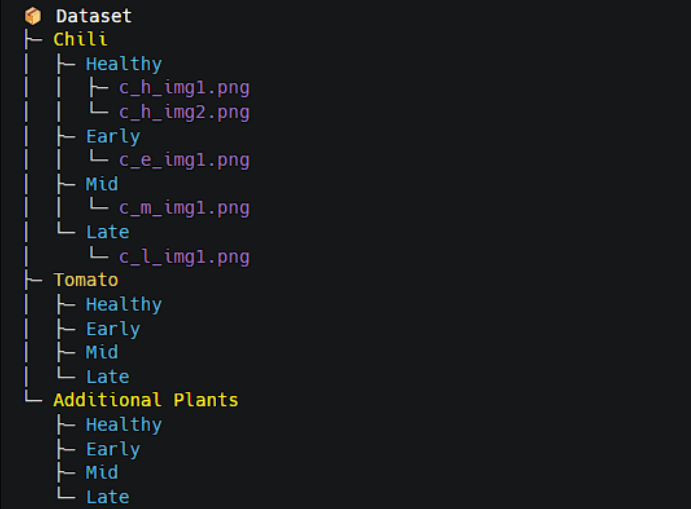
\includegraphics[scale=0.5]{images/ds.png}
    
    \caption{Structure of the dataset}
\end{center}


The foundation of this research rests upon a meticulously curated dataset that combines multiple established plant disease image collections with newly gathered samples. The consolidated dataset integrates images from diverse sources including the Plant-Doc dataset, PlantVillage dataset, iBean dataset, Citrus Leaves dataset, and Rice Leaf Disease dataset, supplemented by direct image collection following standardized guidelines. This comprehensive approach has yielded approximately 21,000 images distributed across 17 distinct plant classes, creating a robust foundation for model training.

\

The dataset structure has been deliberately designed to facilitate seamless integration of new data, with the training folder organized hierarchically according to prediction classes. A notable characteristic of the compiled dataset is its inherent class imbalance, where certain categories contain significantly fewer samples than others. This imbalance, resulting from the heterogeneous nature of the source datasets, presents a long-tail classification challenge that necessitates specialized preprocessing and training methodologies.

\

The preprocessing pipeline has been specifically optimized for Vision Transformer architecture implementation. Given the heterogeneous nature of the source data, with variations in image dimensions, formats, and capture conditions, a standardized preprocessing workflow has been established. Images undergo uniform rescaling and resizing to 224 x 224 resolution before being processed through the ViT preprocessor for patch-wise decomposition. This preprocessing is executed dynamically to maintain dataset integrity across different model architectures, with plans to incorporate disease progression stage data in future iterations.

\

The language modeling component employs the Llama 3.2 2b model, implementing a Retrieval-Augmented Generation (RAG) pipeline to circumvent the computational demands of full model fine-tuning. The knowledge base consists of manually curated information that is embedded and stored in a vector database, enabling semantic and contextual information retrieval during response generation. To optimize system performance, frequently asked questions about specific plant conditions are preemptively provided during prediction, reducing the inference load on the language model.

\

The training methodology follows a two-phase approach. The initial training phase utilizes pre-trained Vision Transformer weights, allowing full network weight updates to optimize performance specifically for plant disease detection. This phase incorporates best weight restoration mechanisms to prevent overfitting, with performance validation conducted on segregated test data. The system implements robust checkpoint saving to enable training resumption in case of interruption. The second phase, balanced retraining, addresses the long-tail classification challenge by training on a balanced dataset with frozen backbone weights. For incorporating new classes, both training phases are repeated using the previously retrained weights as initialization points, ensuring seamless model expansion while maintaining performance integrity.

\

This comprehensive data and training methodology establishes a robust foundation for accurate plant disease detection while maintaining flexibility for future improvements and expansions. The approach effectively addresses common challenges in agricultural image classification while providing a scalable framework for continuous system enhancement.



\subsection{Algorithm/Model Design:}
% Explain the model architecture, algorithmic steps, or computational processes.
\begin{itemize}

\item \textbf{Vision Model:}
\begin{itemize}
\item \textbf{Pretrained Vision Transformer (ViT):} Extracts hierarchical visual features for disease classification.
\item \textbf{Custom CNN Layers:} Fine-tuned layers to improve feature extraction.
\item \textbf{Transfer Learning:} Utilizes pre-trained weights to accelerate training and optimize accuracy.
\end{itemize}

\item \textbf{Language Model:}
\begin{itemize}
\item \textbf{LLaMA 3.2 LLM:} Used for interactive chatbot responses with domain-specific customization.
\item \textbf{RAG Pipeline:} Enhances text generation by integrating document retrieval for contextual answers.
\end{itemize}

\end{itemize}

The classification framework implements a sophisticated multi-stage approach that integrates both visual and linguistic processing components. The visual analysis pipeline begins with advanced feature extraction techniques, where the Vision Transformer architecture processes the input image through its attention mechanisms, effectively identifying and isolating distinctive characteristics of plant diseases. This includes subtle variations in leaf coloration, texture patterns, and structural deformities that may indicate specific pathologies.
Image segmentation plays a crucial role in the detection pipeline, employing region-based analysis to isolate affected areas from healthy plant tissue. This segmentation process enhances the model's ability to focus on disease-specific features while minimizing the impact of background noise and environmental variations. The segmented regions undergo detailed analysis through the transformer's multi-head attention layers, enabling the system to capture both local and global contextual information critical for accurate disease classification.
The natural language processing component leverages semantic similarity search through a carefully structured vector database system. This database stores dense vector embeddings of domain-specific agricultural knowledge, disease characteristics, and treatment protocols. The embedding process transforms textual information into high-dimensional vectors that preserve semantic relationships, enabling the system to perform rapid and contextually relevant information retrieval. When a disease is identified through the visual pipeline, the system can quickly access and retrieve relevant information about the condition, its progression patterns, and recommended treatment approaches.
The integration of these visual and textual processing pipelines creates a comprehensive system that not only identifies plant diseases but also provides meaningful, context-aware recommendations. This unified approach ensures that farmers receive both accurate diagnoses and practical, actionable insights for disease management.

\subsection{Tools and Technologies:} 
% Mention the programming languages, libraries, or software used.System Architecture/Design (Optional, for implementation-based projects)
% Provide a high-level view of the system's components and interactions.
% Include block diagrams or flowcharts to illustrate the design.
% Describe individual components and their roles.

\begin{itemize}

\item \textbf{Programming Languages:}
\begin{itemize}
\item Python, Node.js
\end{itemize}

\item \textbf{Libraries and Frameworks:}
\begin{itemize}
\item TensorFlow, PyTorch, OpenCV, Scikit-learn, Keras
\end{itemize}

\item \textbf{Vector Database:}
\begin{itemize}
\item ChromaDB for storing embeddings
\end{itemize}

\item \textbf{Deployment Tools:}
\begin{itemize}
\item Docker for containerization, Hugging Face for cloud hosting
\end{itemize}

\item \textbf{Mobile Development:}
\begin{itemize}
\item Flutter for cross-platform app development
\end{itemize}

\item \textbf{Version Control:}
\begin{itemize}
\item GitHub repositories for modular development
\end{itemize}

\end{itemize}

The current stage of this project is primarily focused on early development and prototyping, necessitating a cost-efficient and resource-conscious approach to implementation. Given the inherent limitations of free cloud services, the architecture emphasizes a decentralized design to ensure scalability and flexibility. At its core, the system is structured as a network of microservices, each of which is tasked with a specific, well-defined responsibility. This modular approach not only simplifies development and maintenance but also facilitates seamless integration and future scalability. Notably, the system does not mandate users to authenticate or provide any personal information, ensuring privacy and accessibility. Instead, each instance of a prediction operates within its own self-contained context, with all relevant data and results stored locally on the user’s device.

Currently, the prediction and language processing systems are hosted online, offering promising capabilities in addressing the identified problem domain. However, there remains considerable scope for improving their performance and expanding their utility. At this stage, the language model relies on a predefined set of static answers tailored to a limited range of frequently asked questions, specifically focusing on diagnosing a single type of plant disease. Ongoing development efforts aim to transition from this rudimentary setup to a more robust, full-text processing system. The end goal is to deploy this enhanced model across multiple low-resource servers, leveraging freely available hosting solutions to ensure widespread accessibility without incurring significant costs.

\begin{center}
    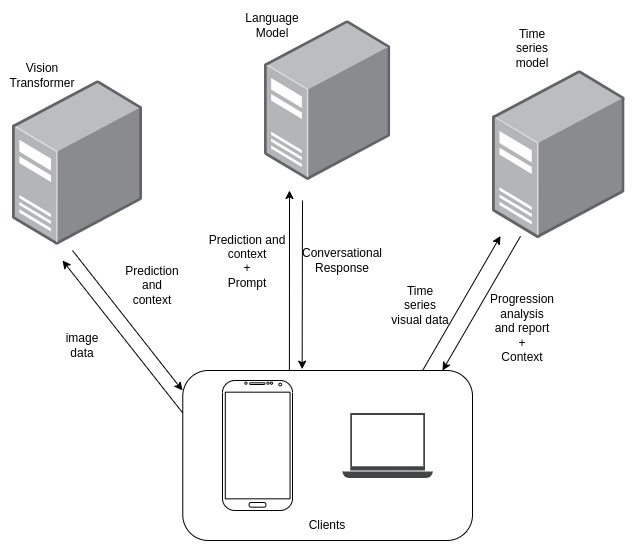
\includegraphics[scale=0.5]{images/architecture.jpg}
    
    \caption{Client-Server Architecture}
\end{center}

\begin{center}
    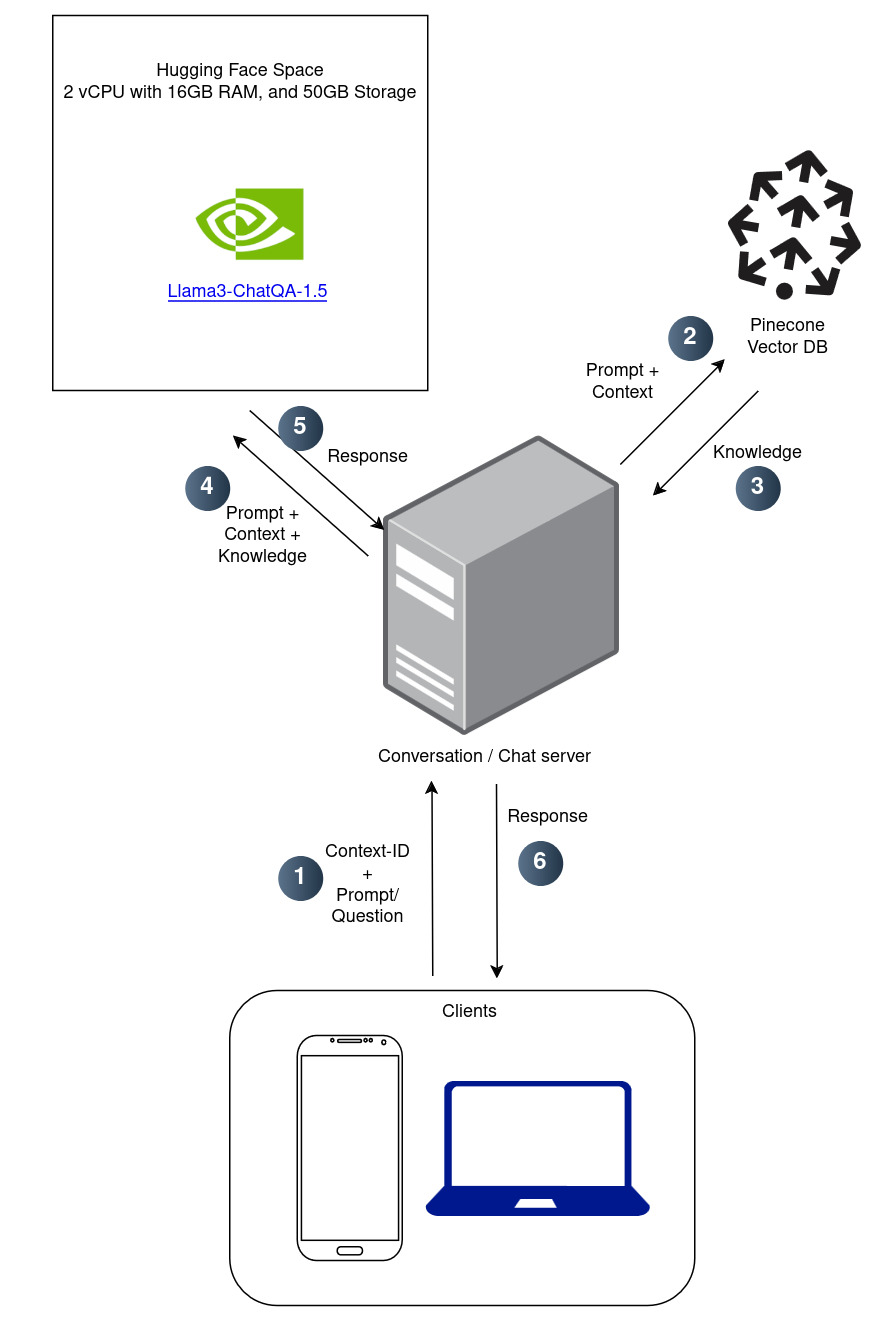
\includegraphics[scale=0.5]{images/chatbot_arch.jpg}
    
    \caption{Chatbot Architecture}
\end{center}

\subsection{Algorithm or Model Description}



% Explain the model architecture, algorithmic steps, or computational processes.

% Also give explanation of how these algorithms are used in solving the problems. The prerequisites, if any, need to be explained.
% Any equations to clarify the algorithms, if necessary, may also be given.\\

The proposed approach for plant disease classification is a multi-stage pipeline designed to ensure high accuracy, robustness, and usability for practical applications. It begins with the input of preprocessed image data, where raw images are standardized through resizing, normalization, and augmentation techniques to enhance model generalization and performance. This preprocessing step addresses variations in lighting, angles, and resolutions, ensuring that the model can handle diverse input conditions effectively.  

Feature extraction is then performed using a Vision Transformer (ViT) architecture, which divides each input image into smaller non-overlapping patches. These patches are subsequently projected into embeddings that preserve spatial and structural information, enabling the model to capture fine-grained details and patterns crucial for disease identification. The ViT leverages self-attention mechanisms, allowing it to model both local and global dependencies within the image data, thus outperforming traditional convolutional neural networks (CNNs) in capturing long-range relationships.  

The training phase employs a fine-tuning approach, where the pre-trained ViT model is adapted to the specific task of plant disease classification. Fine-tuning involves updating the model’s weights using domain-specific datasets, ensuring it learns features that are particularly relevant to plant diseases. To address class imbalances often observed in agricultural datasets, weighted loss functions are incorporated. For binary classification tasks, Binary Cross-Entropy is applied, whereas Categorical Cross-Entropy is used for multi-class classification. These loss functions are optimized using gradient-based methods, ensuring that the model’s predictions align closely with ground-truth labels.  

Validation is an integral part of the pipeline, where the model’s performance is rigorously assessed using multiple evaluation metrics, including accuracy, precision, recall, and F1-score. Accuracy measures overall correctness, precision evaluates the proportion of correctly identified positive cases, recall quantifies the ability to detect positive cases, and F1-score balances precision and recall to provide a holistic performance metric. This stage helps identify potential overfitting or underfitting, guiding further adjustments to the training process.  

Once the model achieves satisfactory performance on validation data, it is deployed to classify new, unseen images. The deployment pipeline is optimized for efficiency, enabling real-time predictions even on low-resource devices. The system outputs the predicted disease class along with confidence scores, providing actionable insights to end-users.  

To improve accessibility and enhance user experience, the solution integrates a chatbot powered by Retrieval-Augmented Generation (RAG). This chatbot serves as an interactive interface, allowing users to query information about plant diseases and receive detailed, context-aware responses. The RAG framework combines the model’s classification results with a database of pre-embedded answers, delivering recommendations on disease management, treatment methods, and preventive measures. This integration ensures that users not only receive predictions but also gain insights into addressing the identified issues effectively.  

From a mathematical standpoint, the model’s optimization process relies on minimizing the specified loss functions. Binary Cross-Entropy, defined as:  

\[
L = -\frac{1}{N} \sum_{i=1}^{N} \left[ y_i \log(p_i) + (1 - y_i) \log(1 - p_i) \right]
\]  

is used for binary classification, while Categorical Cross-Entropy, expressed as:  

\[
L = -\sum_{i=1}^{N} \sum_{j=1}^{C} y_{ij} \log(p_{ij})
\]  

is employed for multi-class scenarios. Here, \( y_i \) and \( p_i \) represent the true and predicted labels, respectively.  

The final layer of the model utilizes the Softmax activation function, given by:  

\[
\sigma(z_i) = \frac{e^{z_i}}{\sum_{j=1}^{C} e^{z_j}}
\]  

where \( z_i \) represents the logits for class \( i \), and \( C \) denotes the number of classes. This function transforms raw logits into probability distributions, enabling the system to determine the most likely disease category.  

In summary, this comprehensive pipeline integrates advanced machine learning techniques, a modular deployment framework, and a chatbot-based recommendation system to deliver an accessible and resource-efficient solution for plant disease classification and management.

The main overview of the entire process is as shown in Algorithnm \ref{alg:cap}

\begin{algorithm}[h]
\caption{PLant Disease Classification }\label{alg:cap}
\begin{algorithmic}[1]
\State \textbf{Input} Image dataset, Target labels\;
\State \textbf{Output} Predicted Values\;
\State Preprocess dataset (resize, normalize)\;
\State Divide image into patches\;
\State Extract features using ViT layers\;
\State Train using fine-tuning approach\;
\State Evaluate model performance on validation set\;
\State Deploy trained model\;

\end{algorithmic} 

\end{algorithm}


%  Provide detailed steps of the proposed algorithm or architecture.
% Outline the algorithm step-by-step.
% Include pseudocode or flowcharts for clarity.
% Explain any mathematical formulations or equations involved.
\subsection{ Expected Outcomes}
% Discuss the anticipated results and how they address the research objectives.
% Highlight the expected performance improvements or practical contributions.

The proposed methodology is built to achieve accuracy and efficiency in the classification of diseases in plants through advanced techniques in machine learning. Advanced machine learning technique will address real-world issues in agriculture. The developed system targets a classification accuracy of over 90% for reliable identification across various species of plants, and its real-time inference capability will make it well-suited for mobile application integration, where speed of result determination is crucial but not less than accuracy in results obtained. The main objective is to ensure low resource requirements, such that deployment is possible even on the edge devices including smartphones and tablets, regardless of how weak the Internet connectivity and computational resources might be. The practical contributions of this solution extend beyond disease detection, offering a comprehensive ecosystem to support farmers and agricultural stakeholders. Central to this ecosystem is a user-friendly mobile application designed to simplify the diagnosis process for farmers. The application provides intuitive navigation and features, allowing users to capture plant images, receive instant diagnoses, and access actionable insights with minimal technical knowledge.

In addition to its diagnostic capability, the system also encompasses a context-aware chatbot based on Retrieval-Augmented Generation (RAG). This chatbot can be thought of as an interactive assistant that provides targeted guidance and remedies according to the disease diagnosed. It fetches information pertinent to pre-trained knowledge bases, which may include treatments, precautions, and viable agricultural techniques. Through the ability of two-way communication, this chatbot also makes accessibility better for the users who can ask clarifications and seek more insight into management techniques of disease.

The proposed solution also supports incremental model updates to ensure long-term adaptability and scalability. This feature allows the system to incorporate new data and expand its knowledge base to include emerging diseases and updated remedies. The model continues to learn from new inputs and stays up-to-date, effectively addressing evolving agricultural challenges without requiring complete retraining.

Overall, this approach is practical, scalable, and accessible for modern agricultural disease management due to its high accuracy, real-time inference, low resource requirements, user-friendly design, and intelligent chatbot integration. It bridges the gap between cutting-edge technology and grassroots farming needs, providing farmers with a reliable tool to safeguard crop health and improve productivity.



\subsection{Advantages of the Proposed Work}
%  Emphasize the benefits of the proposed approach.
% Compare with existing methods, highlighting improvements.
% Mention scalability, efficiency, accuracy, or usability gains.



\subsection{Limitations and Assumptions}
%  Acknowledge potential limitations and assumptions made in the study.

% Mention constraints like computational resources, data availability, or generalizability.
% Discuss any assumptions inherent in the model or methodology.


